\documentclass{standalone}

\usepackage[OT1]{fontenc}
\renewcommand*\familydefault{\sfdefault}
\usepackage{helvet,sfmath}
\usepackage{siunitx}

\usepackage{tikz}
\usetikzlibrary{arrows,calc,patterns}
\usepackage{tikz,tkz-euclide}

\definecolor{BlueDefault}{rgb}{0.2,0.2,0.7}

\begin{document}

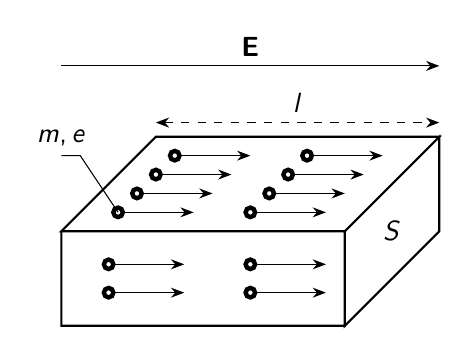
\begin{tikzpicture}[scale=0.6]
        \draw[thick]
        (6,0) to (8,2) to (2,2) to (0,0) to (6,0) to (6,-2) to (8,0) to (8,2) to (6,0) to (6,-2) to (0,-2) to (0,0);
        \draw[dashed, Stealth-Stealth] (2,2.3) to (8,2.3);
        \draw (5,2.3) node[above]{$l$} (7,0) node{\(S\)};
        %%Layer_1
        \draw[-Stealth] (2.4,1.6) to (4.0,1.6);
        \filldraw[color=black, fill=white, ultra thick](2.4,1.6) circle (0.1);
        \draw[-Stealth] (2.0,1.2) to (3.6,1.2);
        \filldraw[color=black, fill=white, ultra thick](2.0,1.2) circle (0.1);
        \draw[-Stealth] (1.6,0.8) to (3.2,0.8);
        \filldraw[color=black, fill=white, ultra thick](1.6,0.8) circle (0.1);
        \draw[-Stealth] (1.2,0.4) to (2.8,0.4);
        \filldraw[color=black, fill=white, ultra thick](1.2,0.4) circle (0.1);
        %%Layer_2
        \draw[-Stealth] (5.2,1.6) to (6.8,1.6);
        \filldraw[color=black, fill=white, ultra thick](5.2,1.6) circle (0.1);
        \draw[-Stealth] (4.8,1.2) to (6.4,1.2);
        \filldraw[color=black, fill=white, ultra thick](4.8,1.2) circle (0.1);
        \draw[-Stealth] (4.4,0.8) to (6.0,0.8);
        \filldraw[color=black, fill=white, ultra thick](4.4,0.8) circle (0.1);
        \draw[-Stealth] (4.0,0.4) to (5.6,0.4);
        \filldraw[color=black, fill=white, ultra thick](4.0,0.4) circle (0.1);
        %%Horizontal_Layer
        \draw[-Stealth] (1.0,-0.7) to (2.6,-0.7);
        \filldraw[color=black, fill=white, ultra thick](1.0,-0.7) circle (0.1);
        \draw[-Stealth] (1.0,-1.3) to (2.6,-1.3);
        \filldraw[color=black, fill=white, ultra thick](1.0,-1.3) circle (0.1);
        \draw[-Stealth] (4.0,-0.7) to (5.6,-0.7);
        \filldraw[color=black, fill=white, ultra thick](4.0,-0.7) circle (0.1);
        \draw[-Stealth] (4.0,-1.3) to (5.6,-1.3);
        \filldraw[color=black, fill=white, ultra thick](4.0,-1.3) circle (0.1);
        %%Note mass and charge
        \draw (1.2,0.4) to (0.4,1.6) to (0,1.6);
        \draw (0,1.6) node[above]{\(m,e\)};
        %%Electric field
        \draw[-Stealth] (0,3.5) to (8,3.5);
        \draw (4,3.5) node[above]{\(\mathbf{E}\)};
        \end{tikzpicture}

\end{document}